\documentclass[10pt]{article}

\usepackage{answers,setspace,graphicx,multicol,enumitem,textcomp}
\usepackage{mathrsfs,svg,adjustbox}
\usepackage[margin=1in]{geometry}
\usepackage{totcount,xcolor,layout,latexsym,times,subfigure}
\usepackage{epsf,prooftrees,natded}
\input{epsf}
\usepackage[normalem]{ulem}
\usepackage{amsmath,amsthm,amssymb,xspace,multirow,graphicx,turnstile, float}
\usepackage[titlenotnumbered,noend,noline]{algorithm2e}

\newcommand{\N}{\mathbb{N}}
\newcommand{\Z}{\mathbb{Z}}
\newcommand{\C}{\mathbb{C}}
\newcommand{\R}{\mathbb{R}}
\newcommand{\Q}{\mathbb{Q}}
\newcommand{\Jas}{Ja\'skowski }
\newcommand{\JasA}{Ja\'skowski}
\newcommand{\KM}{Kalish-Montague }
\newcommand{\KMa}{Kalish-Montague}
\newcommand*{\Co}[2]{{}^{#1}C_{#2}}%

\DeclareMathOperator{\sech}{sech}
\DeclareMathOperator{\csch}{csch}

\newenvironment{theorem}[2][Theorem]{\begin{trivlist}
\item[\hskip \labelsep {\bfseries #1}\hskip \labelsep {\bfseries #2.}]}{\end{trivlist}}
\newenvironment{definition}[2][Definition]{\begin{trivlist}
\item[\hskip \labelsep {\bfseries #1}\hskip \labelsep {\bfseries #2.}]}{\end{trivlist}}
\newenvironment{proposition}[2][Proposition]{\begin{trivlist}
\item[\hskip \labelsep {\bfseries #1}\hskip \labelsep {\bfseries #2.}]}{\end{trivlist}}
\newenvironment{lemma}[2][Lemma]{\begin{trivlist}
\item[\hskip \labelsep {\bfseries #1}\hskip \labelsep {\bfseries #2.}]}{\end{trivlist}}
\newenvironment{exercise}[2][Exercise]{\begin{trivlist}
\item[\hskip \labelsep {\bfseries #1}\hskip \labelsep {\bfseries #2.}]}{\end{trivlist}}
\newenvironment{solution}[2][Solution]{ \begin{trivlist}
\item[\hskip \labelsep {\bfseries #1}]}{\end{trivlist}}
\newenvironment{problem}[2][Problem]{\begin{trivlist}
\item[\hskip \labelsep {\bfseries #1}\hskip \labelsep {\bfseries #2.}]}{\end{trivlist}}
\newenvironment{question}[2][Question]{\begin{trivlist}
\item[\hskip \labelsep {\bfseries #1}\hskip \labelsep {\bfseries #2.}]}{\end{trivlist}}
\newenvironment{corollary}[2][Corollary]{\begin{trivlist}
\item[\hskip \labelsep {\bfseries #1}\hskip \labelsep {\bfseries #2.}]}{\end{trivlist}}

\begin{document}

% --------------------------------------------------------------
%                         Start here
% --------------------------------------------------------------

\title{Assignment 3}%replace with the appropriate homework number
\author{Aditya Arora\\ %replace with your name
Winter 2018\\$Quidquid\ Latine\ dictum\ sit,\ altum\ viditur$} %if necessary, replace with your course title
\maketitle

%Below is an example of the problem environment
\begin{problem}{1}
If you roll a fair dice $n$ times:
\begin{enumerate}[label=(\alph*)]
    \parskip=0in
    \parsep=0in
    \itemsep=0.1in
    \item In how many ways will you always get all six numbers at least once, assuming $n \geq 6$? What is the probability of this occurring?
    \item In how many ways will the sum of the number of 1’s and 2’s equal the sum of the number of 3’s, 4’s, 5’s and 6’s, assuming $n= 2i$ for some positive integer $i$? What is the probability of this occurring?
    \item In how many ways will the sum of the number of 1’s and 2’s equal the sum of the number of 3’sand 4’s and equal the sum of the number of 5’s and 6’s, assuming $n= 3i$ for some positive integer $i$? What is the probability of this occurring?
    \item In how many ways will you roll a \textquotedblleft1\textquotedblright \ at least twice among all n dice rolls, assuming $n \geq 2$? What is the probability of this occurring?
    \item In how many ways will you roll a \textquotedblleft1\textquotedblright \ at least $k$ times, assuming $n \geq k$? What is the probability of this occurring?
    \item You have a communications system that transmits bundles of data from a source to a destination. Most bundles are received correctly. However, there is a random chance of the data in a bundle being in error. Roughly every $E^{th}$ bundle is in error. If you transmit $n$ bundles, what is the probability of at least two bundles being in error? what is the probability of at least $k$ bundles being in error?
    % \item In how many ways will you roll a “1” twice in succession at least once, assuming $n \geq 2$? What is the probability of this occurring?
    % \item In how many ways will you roll a \textquotedblleft1\textquotedblright \ k-times in succession at least once, assuming $n \geq k$? What is the probability of this occurring?
    % \item You have a communications system that transmits bundles of data from a source to a destination. Most bundles are received correctly. However, there is a random chance of the data in a bundle being in error. Roughly every $E^{th}$ bundle is in error. If you transmit $n$ bundles, what is the probability of at least two bundles in sequence being in error? what is the probability of at least $k$ bundles in sequence being in error?
\end{enumerate}

You may wish to modify your Lab3 program {\tt dice} to give you a
sense of whether or not your answers look correct.
\end{problem}

%Below is the solution environment
\begin{solution}{1}
\item[]
    $$\textbf{Proof for: }{n \choose 0} + {n \choose 1} + ... + {n \choose n} = 2^n\textbf{  Proof (1)}$$

    For basic step n=0:
    $\binom{0}{0}=\frac{0!}{0!0!}=2^0$

    For induction step:
    Let k be an integer such that $0 < {k}$ and for all L, $0\le{L}\le{k}$ where $L\in{I}$, the formula stand true.
    Then let the following statement be trueh:
    $$\binom{k}{0}+\binom{k}{1}+...+\binom{k}{k}=2^k$$
    Now as can be illustrated easily $\binom{k}{0}=\binom{k+1}{0}$ and $\binom{k}{k}=\binom{k+1}{k+1}$.
    Now by using Pascal's identity,
    $$
        \binom{k+1}{0}+\binom{k+1}{1}+\binom{k+1}{2}+...+\binom{k+1}{k}+\binom{k+1}{k+1}\\$$ $$
        =\binom{k+1}{0}+\binom{k}{0}+\binom{k}{1}+\binom{k}{1}+\binom{k}{2}+...+\binom{k}{k-1}+\binom{k}{k}+\binom{k+1}{k+1}\\ $$ $$
        =\binom{k}{0}+\binom{k}{0}+\binom{k}{1}+\binom{k}{1}+\binom{k}{2}+...+\binom{k}{k-1}+\binom{k}{k}+\binom{k}{k}\\ $$ $$
        =2*{\sum_{i=0}^k\binom{k}{i}}\\=2*2^k\\=2^{k+1}
    $$
    As the formula is also true for $k+1$ hence by second principle of finite induction this formula is valid for all integers greater than or equal to $0$.\\
\begin{enumerate}[label=(\alph*)]
    \parskip=0in
    \parsep=0in
    \itemsep=0.1in
    \item Let $E$ be the event such that you get all six numbers at least once. $E'$ is the event such that you never get all 6 numbers. Since $E$ and $E'$ are complimentary events we can safely say that $$P(E) + P(E') = 1$$ where $P(x)$ is the probability of an event $x$ occurring.

    Number of time $E'$ occurs = Total number of cases($6^n$) - Number of time $E$ occurs\\
    We now need to find out the number of times $E'$ occurs. It can be such that:
    \begin{enumerate}[label=(\Roman*)]
    \parskip=0in
    \parsep=0in
    \itemsep=0.1in
    \item Only one number occurs $n$ total times:\\
        There are only 6 such cases where only one of the numbers occurs
    \item Only two numbers occur $n$ total times:\\
        Out of the 6 numbers on a dice we can select two of them to show up, we can then permute their arrangements.\\
        So we first select 2 out of the 6 numbers: $\Co{6}{2}$.\\
        Then we need to find the number of their permutations which works out to $2^n$ because for each roll we basically have to choose between the 2 numbers.\\
        Therefore the total number of cases is $\Co{6}{2} 2^n$
    \item Only three numbers occur $n$ total times:\\
        Similar to when we have two numbers: We first select 3 out of the 6 numbers $\Co{6}{3}$ and then permute them $3^n$ ways which works out to $\Co{6}{3} 3^n$ total cases
    \item Only four numbers occur $n$ times: \\
        Similar to when we have two numbers: We first select 4 out of the 6 numbers $\Co{6}{4}$ and then permute them $4^n$ ways which works out to $\Co{6}{4} 4^n$ total cases
    \item Only five numbers occur $n$ times:\\
        Similar to when we have two numbers: We first select 5 out of the 6 numbers $\Co{6}{5}$ and then permute them $4^n$ ways which works out to $\Co{6}{5} 5^n$ total cases
    \end{enumerate}
        Adding all these cases up we get the total number of time $E'$ can occur as: $6+\Co{6}{2} 2^n+\Co{6}{3} 3^n+\Co{6}{4} 4^n+\Co{6}{5} 5^n$\\
        $$ 15*2^n + 15*2^{2n} + 20*3^n + 6*5^n + 6 $$
    The total number of cases = $6^n$
    Thus the total number of occurrences possible of $E$ are \\$6^n - {(15*2^n + 15*2^{2n} + 20*3^n + 6*5^n + 6)}$\\
    Thus $$P(E) = \frac{6^n - {(15*2^n + 15*2^{2n} + 20*3^n + 6*5^n + 6)}}{6^n}$$
    \item We know that $n=2i \Rightarrow i = n/2$, half of the positions are filled with $1's$ and $2's$ while the rest are filled with $3's,\ 4's,\ 5's$ and $6's$\\
    So for $1's$ and $2's$: There are $n/2$ places out of the $n$ places possible that are filled with $1's$ and $2's$.\\
    So for filling those $i$ places:\\
    We can select $r$ places out of the $i$ places to fill with $1's$ and the rest with $2's$. We can then change $r$ from $0$ to $i$ to account for all possible combinations of $1's$ and $2's$\\
    $$\sum_{r=0}^{i} \Co{i}{r} = 2^i\ \ \ \ \ \ \  \text{           [Using Proof(1)]}$$
    Therefore we now know that for having $1's$ and $2's$ in $i=n/2$ places the possible combinations are $=2^{i}$
    For filling out the remaining places with $3's,\ 4's,\ 5's$ and $6's$\\
    Let $j$ places out of the remaining $i$ places be filled with $3's$, $k$ out of the remaining $i-j$ places be filled with $\ 4's,$ and lastly $l$ out of the remaining $i-j-k$ be filled with $\ 5's$. All the remaining $i-j-k-l$ places can be filled with $\ 6's$\\
    We can then change $l$ from $0$ to $k$, $k$ from $0$ to $j$ and $j$ from $0$ to $i$ to account for all possible combinations of $3's,\ 4's,\ 5's$ and $6's$\\
    $$\sum_{j=0}^{i} \sum_{k=0}^{j} \sum_{l=0}^{k} \Co{i}{j}  \Co{i-j}{k} \Co{i-j-k}{l}$$
    $$\sum_{j=0}^{i} \sum_{k=0}^{j} \sum_{l=0}^{k} \Co{i}{j}  \Co{i-j}{k} \Co{i-j-k}{l}$$
    $$= \sum_{j=0}^{i} \sum_{k=0}^{j} \Co{i}{j}  \Co{i-j}{k}\ 2^{i-j-k}\ \ \ \ \ \ \ \ \ \ \  \text{                   [Using Proof(1)]}$$\\
    Now using Binomial Theorem twice $( (1+x)^n = \sum_{k=0}^n {n \choose k}  x^k ) ]$
    $$= \sum_{j=0}^{i} \Co{i}{j}\ 3^{i-j}$$
    $$=4^{i}$$
    Therefore we now know that for having $3's,\ 4's,\ 5's$ and $6's$ in $i=n/2$ places the possible combinations are $=4^{i}$  \\
    Now we just have to select $n/2$ places out of the given $n$ places and fill those with $1's$ and $2's$, the remaining $n/2$ places can be filled automatically with $3's,\ 4's,\ 5's$ and $6's$.\\
    Therefore for arranging the $1's$ and $2's$ we have $\Co{n}{\frac{n}{2}} 2^{\frac{n}{2}}$ combinations. But for each such case there are $4^i$ arrangements of $3's,\ 4's,\ 5's$ and $6's$\\
    Therefore the total number of combinations is: $\Co{n}{n/2} 2^{\frac{n}{2}} 4^{\frac{n}{2}}$ which on simplification yields: $\Co{n}{\frac{n}{2}} 2^{\frac{3n}{2}}$

     $$P(E) = \frac{\Co{n}{\frac{n}{2}} 2^{\frac{3n}{2}}}{6^n}$$

    \item We know that $n=3i \Rightarrow i = n/3$, one third of the positions are filled with $1's$ and $2's$, another one third of the positions are filled with $3's,\ 4's$ while the rest are filled with $5's$ and $6's$\\
    So for $1's$ and $2's$: There are $n/3$ places out of the $n$ places possible that are filled with $1's$ and $2's$.\\
    So for filling those $i$ places:\\
    We can select $r$ places out of the $i$ places to fill with $1's$ and the rest with $2's$. We can then change $r$ from $0$ to $i$ to account for all possible combinations of $1's$ and $2's$\\
    $$\sum_{r=0}^{i} \Co{i}{r} = 2^i\ \ \ \ \ \ \  \text{           [Using Proof(1)]}$$
    Therefore we now know that for having $1's$ and $2's$ in $i=n/3$ places the possible combinations are $=2^{i}$
    Similarly for arranging $3's,\ 4's$ in $i$ positions we get $2^{i}$ arrangements. Similarly for $5's$ and $6's$ we get $2^{i}$ arrangements.\\

    Now we just have to select $n/3$ places out of the given $n$ places and fill those with $1's$ and $2's$, another $n/3$ places can be filled automatically with $3's,\ 4's$ the remaining positions can be filled $\ 5's$ and $6's$.\\
    Therefore for arranging the $1's$ and $2's$ we have $\Co{n}{\frac{n}{3}} 2^{\frac{n}{3}}$ combinations. But for each such case there are $2^i$ arrangements of $3's,\ 4's$ and another $2^{\frac{n}{3}}$ $5's$ and $6's$\\
    This means we have to select another $n/3$ positions to fill with $3's,\ 4's$, the rest can be then filled with $5's$ and $6's$. This leads to: $\Co{n}{n/3} \Co{2n/3}{n/3} 2^{\frac{n}{3}} 2^{\frac{n}{3}} 2^{\frac{n}{3}}$\\
    Therefore the total number of combinations is: $\Co{n}{n/3} \Co{2n/3}{n/3} 2^{\frac{n}{3}} 2^{\frac{n}{3}} 2^{\frac{n}{3}}$ which on simplification yields: $\Co{n}{n/3} \Co{2n/3}{n/3} 2^{n}$ $$P(E) =\frac{n!*2^n}{(i!)^3 * 6^n}$$
    \item Let $E$ be the event such that you get all \textquotedblleft1\textquotedblright \ occurs at least twice. $E'$ is the event such that you \textquotedblleft1\textquotedblright \ doesn't occur at least twice. Since $E$ and $E'$ are complimentary events we can safely say that $$P(E) + P(E') = 1$$ where $P(x)$ is the probability of an event $x$ occurring.

    Number of time $E'$ occurs = Total number of cases($6^n$) - Number of time $E$ occurs\\
    We now need to find out the number of times $E'$ occurs. It can be such that:
    \begin{enumerate}[label=(\Roman*)]
    \parskip=0in
    \parsep=0in
    \itemsep=0.1in
    \item \textquotedblleft1\textquotedblright \ occurs only once:\\
        Out of the $n$ rolls if \textquotedblleft1\textquotedblright \ occurs only once then there are only $\Co{n}{1} = n$ such selections but each such selection has $5^{n-1}$ choices for the remaining dice rolls
        Therefore total selections: $n5^{n-1}$
        % from the $n$ rolls where \textquotedblleft1\textquotedblright \ occurs only once.
    \item \textquotedblleft1\textquotedblright \ never occurs:\\
        If \textquotedblleft1\textquotedblright \ never occurs then we can say that each of the $n$ rolls can either be $2$ or $3$ or $4$ or $5$ or $6$. This means that each roll has 5 options which means that total such cases are $5^n$
    \end{enumerate}
    Thus the total number of cases for $E$ are $6^n - E'$, which means total cases for E are: $6^n - 5^n - (n5^{n-1})$
    $$P(E) = \frac{6^n - 5^n - (n5^{n-1})}{6^n}$$

    \item Let $E$ be the event such that you get all \textquotedblleft1\textquotedblright \ occurs at least k times. $E'$ is the event such that you \textquotedblleft1\textquotedblright \ doesn't occur at least k times. Since $E$ and $E'$ are complimentary events we can safely say that $$P(E) + P(E') = 1$$ where $P(x)$ is the probability of an event $x$ occurring.

    Number of time $E'$ occurs = Total number of cases($6^n$) - Number of time $E$ occurs\\
    We now need to find out the number of times $E'$ occurs. It can be such that:
    \begin{enumerate}[label=(\arabic*)]
    \parskip=0in
    \parsep=0in
    \itemsep=0.1in
    \item \textquotedblleft1\textquotedblright \ occurs only $k-1$ times: \\
    Select $k-1$ positions and fill them with ones, the rest positions can be filled with any number from $2$ to $5$. Thus total such cases come out to be:\\
        $\Co{n}{k-1} * 5^{n-k+1}$
    \item \textquotedblleft1\textquotedblright \ occurs only $k-2$ times:\\
    Select $k-2$ positions and fill them with ones, the rest positions can be filled with any number from $2$ to $5$. Thus total such cases come out to be:\\
        $\Co{n}{k-2} * 5^{n-k}$
    \item $\dotsb$
    \item[(k)] \textquotedblleft1\textquotedblright \ occurs only once:\\
        Out of the $n$ rolls if \textquotedblleft1\textquotedblright \ occurs only once then there are only $\Co{n}{1} = n$ such selections but each such selection has $5^{n-1}$ choices for the remaining dice rolls
        Therefore total selections: $n5^{n-1}$
        % from the $n$ rolls where \textquotedblleft1\textquotedblright \ occurs only once.
    \item[(k+1)] \textquotedblleft1\textquotedblright \ never occurs:\\
        If \textquotedblleft1\textquotedblright \ never occurs then we can say that each of the $n$ rolls can either be $2$ or $3$ or $4$ or $5$ or $6$. This means that each roll has 5 options which means that total such cases are $5^n$
    \end{enumerate}
    The total cases for $E'$ are $\sum_{r=0}^{k-1} \Co{n}{r} * 5^{n-r}$ \\
    Thus the total number of cases for $E$ are $6^n - E'$, which means total cases for E are: $6^n - \sum_{r=0}^{k-1} \Co{n}{r} * 5^{n-r}$
    $$P(E) = \frac{6^n - \sum_{r=0}^{k-1} \Co{n}{r} * 5^{n-r}}{6^n}$$

    \item
    % You have a communications system that transmits bundles of data from a source to a destination. Most bundles are received correctly. However, there is a random chance of the data in a bundle being in error. Roughly every $E^{th}$ bundle is in error. If you transmit $n$ bundles, what is the probability of at least two bundles being in error? What is the probability of at least $k$ bundles being in error?\\\\


    % Probability that a bundle is in error $= 1/E$ and probability that it does not error is $= (E-1)/E$. Let $R$ be the event such that you get at least 2 bundles are in error $= 1/E$ and the probability for \\$R'$ is $=1- (1/E) = (E-1)/E$. $R'$ is the event such that you less than two bundles are in error. Since $R$ and $R'$ are complimentary events we can safely say that $$P(R) + P(R') = 1$$ where $P(x)$ is the probability of an event $x$ occurring.

    % Number of time $R'$ occurs = Total number of cases($2^N$) - Number of time $R$ occurs\\
    % We now need to find out the number of times $R'$ occurs. It can be such that:
    % \begin{enumerate}[label=(\Roman*)]
    % \parskip=0in
    % \parsep=0in
    % \itemsep=0.1in
    % \item Only $k-1$ errors:\\
    %     Out of the $n$ bundles if only $k$ error-ed then we select $k$ out of the $n$ which we can consider to be the error bundles. The probability of that occurring is
    % \item Only one bundles errors:\\
    %     Out of the $n$ transmitted bundles if only one bundle error-ed then it could be any one of the $n$ bundles. Therefore total such cases $=\Co{n}{1} = n$. Therefore the probability of this occuring is $= (\frac{E-1}{E})^{^{n-1}}$ since all but one bundle did not error
    % \item No bundle errors:\\
    %     There is only one case where no bundle errors and the probability of that occurring is $= (\frac{E-1}{E})^{^{n}}$ because none of the bundle error-ed.
    % \end{enumerate}
    % Therefore the probability of event $E'$ is $= (\frac{E-1}{E})^{^{n-1}} + (\frac{E-1}{E})^{^{n}}$ which implies that the probability of $E$ is $1 - P(E) = 1 - (\frac{E-1}{E})^{^{n-1}} + (\frac{E-1}{E})^{^{n}}$
    % \\\\
    % Thus, the total number of occurences $P(E) * \text{Total events} (2^n) = (1 - (\frac{E-1}{E})^{^{n-1}} + (\frac{E-1}{E})^{^{n}}) * 2^n$
    Let’s say the bundle is like a $E$-sided dice, if we roll a $E$, we get error
    \begin{enumerate}[label=(\arabic*)]
    \parskip=0in
    \parsep=0in
    \itemsep=0.1in
    \item Total size when there are zero errors:  $\Co{n}{0} (E - 1)^n$ \item Total size when there is exactly one errors:  $\Co{n}{1} (E - 1)^{n-1}$
    \item Total size when there are exactly 2 errors:  $\Co{n}{2} (E - 1)^{n-2}$
    \item $\dotsb$
    \item[(k)] Total size when there are exactly k-1 errors:  $\Co{n}{k-1} (E - D1)^{n-k+1 }$
    \end{enumerate}
    Probability for at least 2 errors: $$\frac{E^n - \sum^{1}_{r=0}\Co{n}{i}(E-1)^{n-i}}{E^n}$$
    Probability for at least $k$ errors: $$\frac{E^n - \sum^{k-1}_{r=0}\Co{n}{i}(E-1)^{n-i}}{E^n}$$
\end{enumerate}
\end{solution}



\vskip 0.5in
\newpage
\begin{problem}{2}
Prove (using induction) the binomial theorem:
\[
(x+a)^n = \sum_{r=0}^n{^{n}C_{r}}\ x^{n-r}a^r
\]
\end{problem}
\begin{solution}{2}
\item[]
$$\binom{n}{r} = {^{n}C_{r}}$$
Pascal's Law: $\binom{n}{r}=\binom{n-1}{r}+\binom{n-1}{r-1}$, where $n$ and $r$ are each $\ge 1$. Expressing the right-hand side in terms of factorials, we get
$$\frac{(n-1)!}{r!(n-r-1)!}+\frac{(n-1)!}{(r-1)!(n-r)!}.$$
We want to bring the above expression to a common denominator. So we multiply top and bottom of the first term by $n-r$, and top and bottom of the second term by $r$. We get
$$\frac{(n-1)!(n-r)+(n-1)!r}{k!(n-r)!}.$$
The bottom now looks nice. The two terms on top have a common factor of $(n-1)!$. So the numerator can be rewritten as
$$(n-1)![(n-r)+r)],$$
which is $(n-1)!n$, that is, $n!$. Thus we end up with $\frac{n!}{r!(n-r)!}$, which is $\binom{n}{r}$.

Thus \textbf{Pascal's Law} is true: $\binom{n}{r}=\binom{n-1}{r}+\binom{n-1}{r-1}$\\
Now for proving the Binomial Theorem
\[
P(y) = (x+a)^y = \sum_{r=0}^y{^{y}C_{r}}\ x^{y-r}a^r\]
We will first see if $P(1)$ is true
\[
P(1) = (x+a)^1 = x^1 + a^1 = \sum_{r=0}^1{^{1}C_{r}}\ x^{1-r}a^r
\]
Thus we can see that $P(1)$ is True

Let us assume that $P(m)$ is true. This means that
\[P(m)  = (x+a)^m = \sum_{r=0}^m{^{m}C_{r}}\ x^{m-r}a^r
\]
Now using $P(m)$ we will try to prove $P(m+1)$\\
We know $P(m) * (x+a) = P(m+1)$\\
Thus: \[P(m+1) = {\sum_{r=0}^m{^{m}C_{r}}\ x^{m-r}a^r } * (x+a) \]
\[\Rightarrow P(m+1) = {\sum_{r=0}^m{^{m}C_{r}}\ x^{m+1-r}a^r } + {\sum_{r=0}^m{^{m}C_{r}}\ x^{m-r}a^{r+1} } \]
\[\Rightarrow P(m+1) = {\sum_{r=0}^m{^{m}C_{r}}\ x^{m+1-r}a^r } + {\sum_{r=1}^m{^{m}C_{r-1}}\ x^{m+1-r}a^{r} } \]
\[\Rightarrow P(m+1) = {{^{m}C_{0}}\ x^{m+1}a^0}+  {\sum_{r=1}^m{^{m}C_{r}}\ x^{m+1-r}a^r } + {\sum_{r=1}^m{^{m}C_{r-1}}\ x^{m+1-r}a^{r} }\]
$$[\text{Re-indexing the sum}]$$
\[\Rightarrow P(m+1) = {{^{m+1}C_{0}}\ x^{m+1}a^0}+  {\sum_{r=1}^m({^{m}C_{r}}\ x^{m+1-r}a^r + {^{m}C_{r-1}}\ x^{m+1-r}a^{r}}) \]
$$[{^{m}C_{0}} = {^{m+1}C_{0}} = 1]$$
\[\Rightarrow P(m+1) = {{^{m+1}C_{0}}\ x^{m+1}a^0}+  {\sum_{r=1}^m({^{m}C_{r}}+ {^{m}C_{r-1}})\ x^{m+1-r}a^r} \]
\[\Rightarrow P(m+1) = {{^{m+1}C_{0}}\ x^{m+1}a^0}+  {\sum_{r=1}^m{^{m+1}C_{r}}\ x^{m+1-r}a^r} \]
$$[\textbf{Pascal's Law: }{^{m}C_{r-1}} + {^{m}C_{r}} = {^{m+1}C_{r}}]$$
\[\Rightarrow P(m+1) = {\sum_{r=0}^m{^{m+1}C_{r}}\ x^{m+1-r}a^r} \]
$$[Re-indexing\ the\ sum]$$\\

Thus we have shown that if $P(m)$ is true we can show that $P(m+1)$ is True. \\

Thus we can say that using the principal of mathematical induction that $
(x+a)^n = \sum_{r=0}^n{^{n}C_{r}}\ x^{n-r}a^r
$ is True


\end{solution}


\pagebreak
\pagebreak
\newpage
\clearpage
\begin{problem}{3}
Is there
\begin{enumerate}[label=(\alph*)]
    \parskip=0in
    \parsep=0in
    \itemsep=0.1in
    \item a graph with 5 vertices and 3 edges?
    \item a graph with 5 odd-degree vertices with 3 edges?
    \item a connected graph with 5 vertices and 3 edges?
    \item a directed graph with 5 vertices and 3 edges?
    \item a disconnected graph (a graph that is not connected) with 5
vertices and 7 edges?
    \item a disconnected, directed graph with 5 vertices and 7 edges?
    \item a graph with 3 vertices and 5 edges?
    \item a directed graph with 3 vertices and 5 edges?
\end{enumerate}

In each case, if there exists such a graph, illustrate it; if not, explain (precisely) why not.
\end{problem}
\begin{solution}{3}
\item[]
\begin{enumerate}[label=(\alph*)]
\item Yes there is a graph with 5 vertices and 3 edges \\ 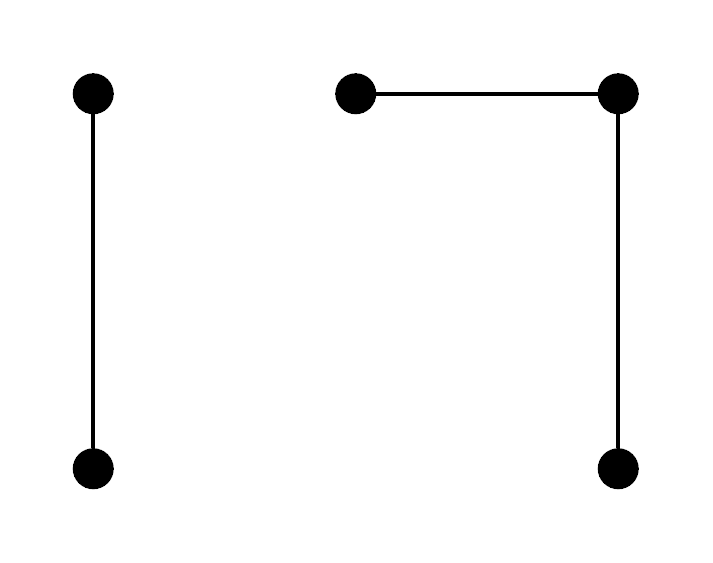
\includegraphics[width=4cm]{graph1}
\item No there does not exist a graph with 5 odd-degree vertices because the sum of all degrees is always even (because the sum of all the degrees is equal to twice the number of edges), but with 5 odd-degree vertices the sum would be odd.
\item No there does not exist a connected graph with 5 vertices and 3 edges because every connected graph with v vertices needs to have at least v - 1 edges
\item Shown below is a graph that is a directed graph with 5 vertices and 3 edges \begin{figure}[H]
    \centering
    \caption{Directed graph with 5 vertices and 3 edges}
    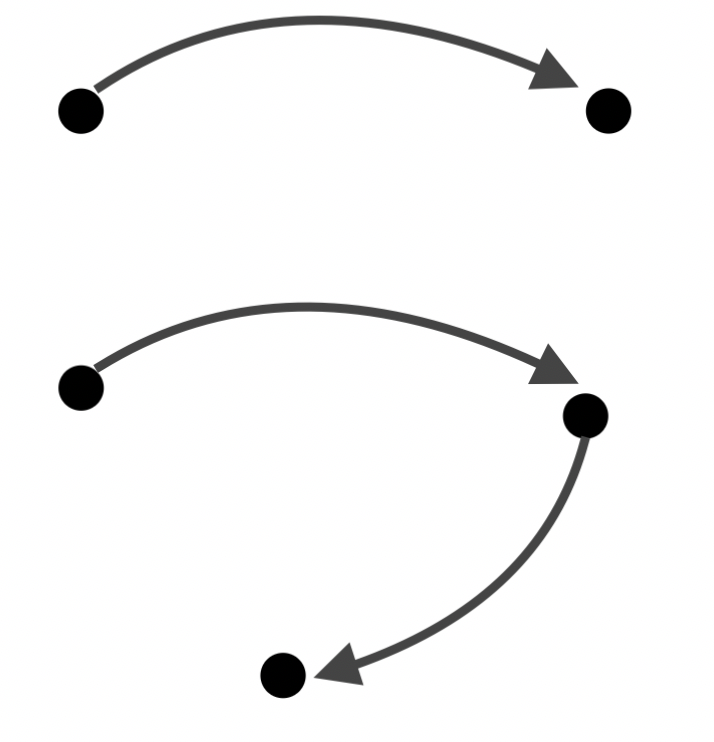
\includegraphics[width=4cm]{graph7}
\end{figure}
\item \pagebreak
No there does not exist a dis-connected graph with 5 vertices and 7 edges. If we try to use 4 connected vertices and 1 disconnected vertex, we only end up with 6 edges\\
\begin{figure}[H]
    \centering
    \caption{Graph with 4 connected vertices}
    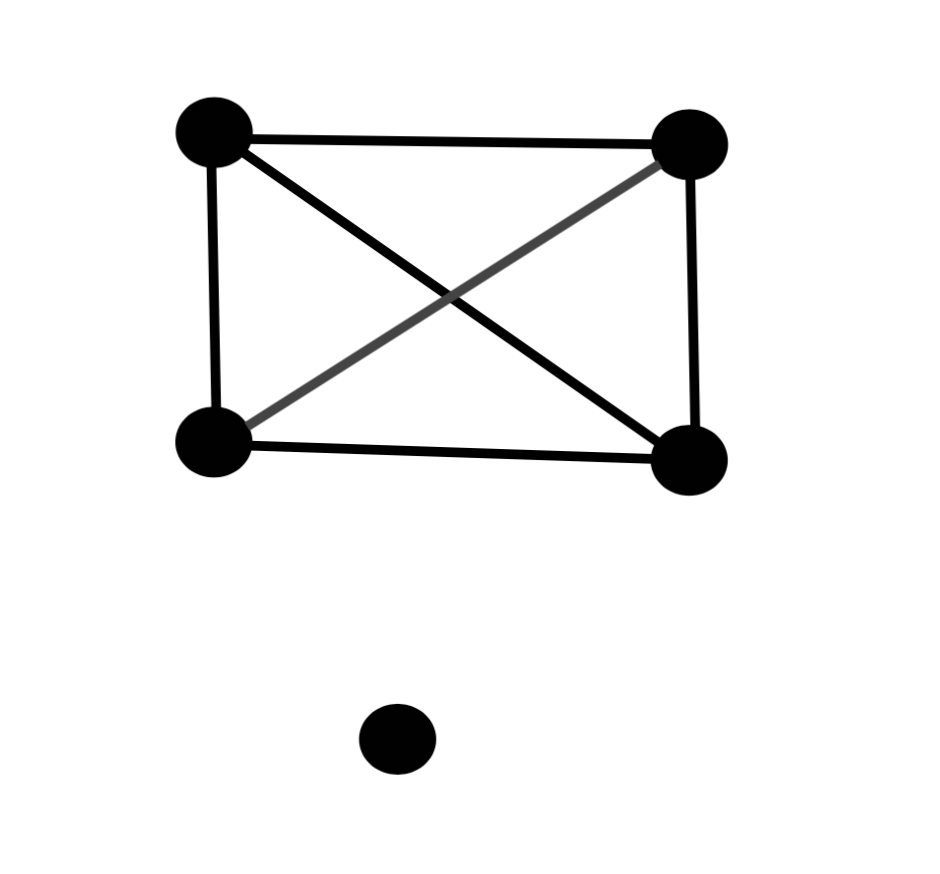
\includegraphics[width=4cm]{graph2}
\end{figure}
If we use 2 connected components, one with 3 connected vertices and one with 2 connected vertices. We still end up with 4 edges\\
\begin{figure}[H]
    \centering
    \caption{Graph with 2 connected components}
    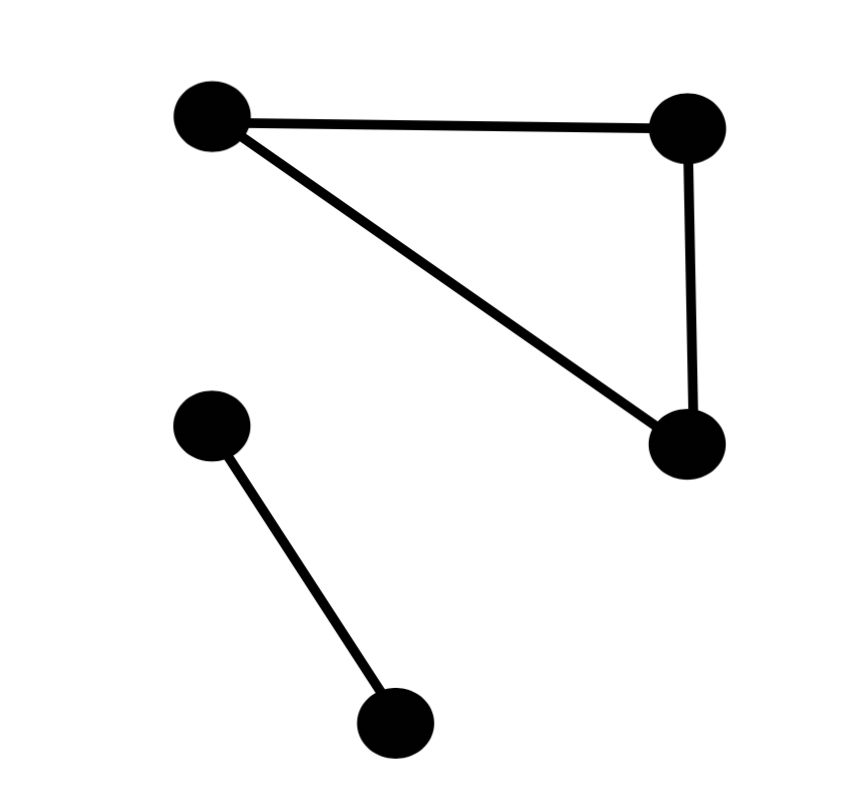
\includegraphics[width=4cm]{graph3}
\end{figure}

If we move to 3 connected components we get only 2 edges
\begin{figure}[H]
    \centering
    \caption{Graph with 3 connected components}
    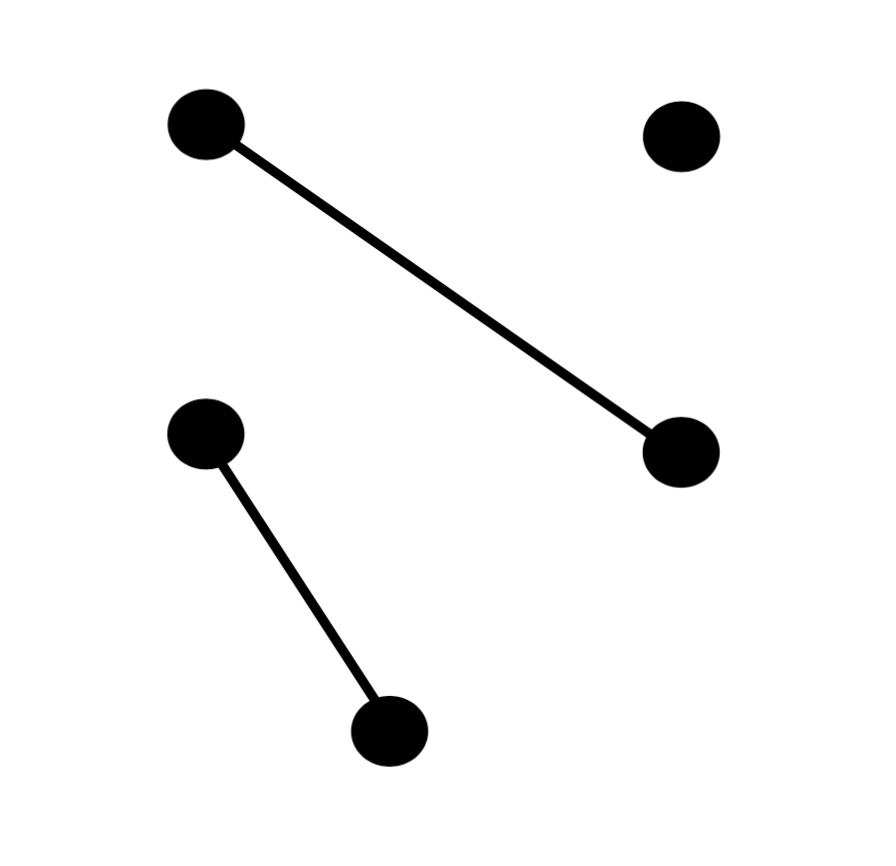
\includegraphics[width=4cm]{graph4}
\end{figure}
\item Shown below is a graph that is disconnected, directed graph and has 5 vertices and 7 edges
\begin{figure}[H]
    \centering
    \caption{a disconnected, directed graph with 5 vertices and 7 edges}
    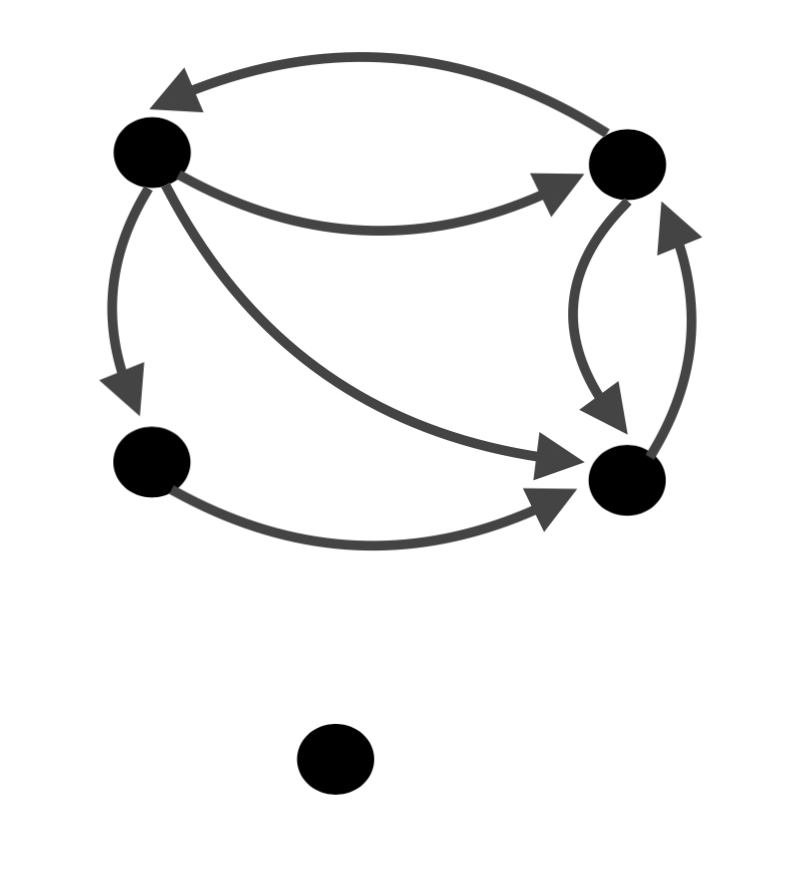
\includegraphics[width=4cm]{graph5}
\end{figure}
\item No there does not exist a graph with 3 vertices and 5 edges. The maximum number of edges possible are $^3C_2 = 3$
\item Shown below is a graph that is a directed graph with 3 vertices and 5 edges
\begin{figure}[H]
    \centering
    \caption{a directed graph with 3 vertices and 5 edges}
    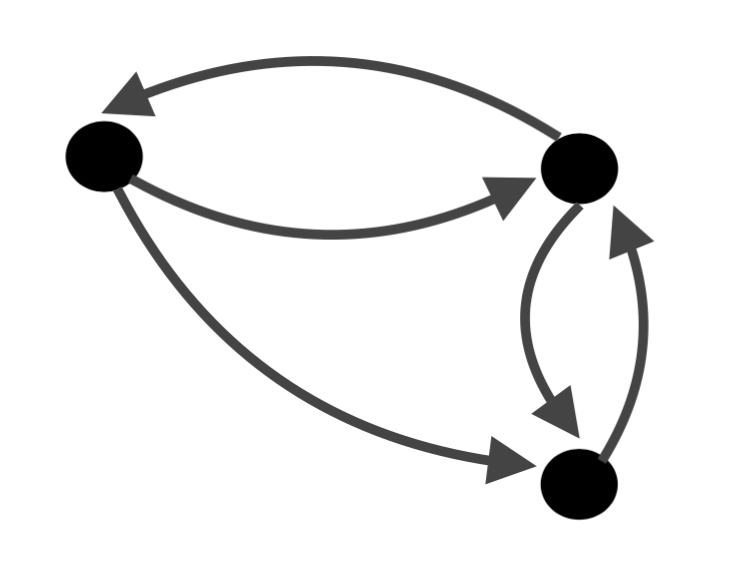
\includegraphics[width=4cm]{graph6}
\end{figure}

\end{enumerate}
\end{solution}

\vskip 0.5in
\newpage
\pagebreak
\pagebreak\newpage

\begin{problem}{4} Given the following graph:

\begin{center}
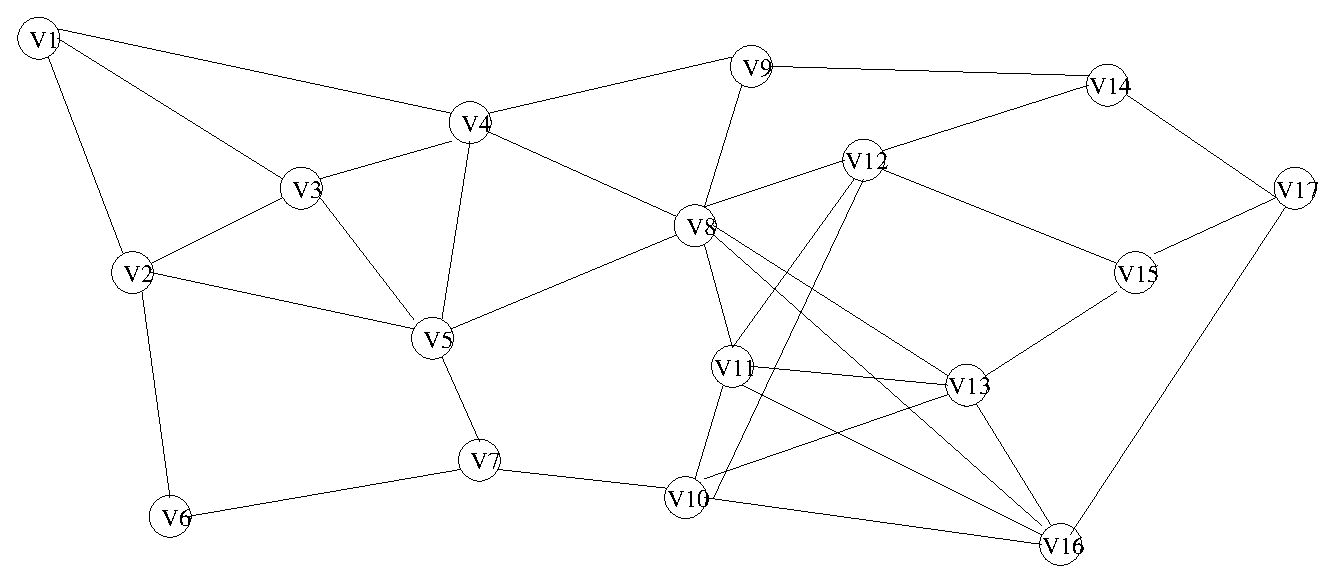
\includegraphics[scale=0.7]{graph.eps}
\end{center}
\begin{enumerate}[label=(\alph*)]
    \parskip=0in
    \parsep=0in
    \itemsep=0.1in
    \item Is this graph connected?
    \item Is this graph complete?  Why/Why not?
    \item What is the minimum degree of the graph?
    \item What is the maximum degree of the graph?
    \item What is the largest clique in the graph?
    \item Is the graph planar? Why/Why not?
    \item What is the shortest path from V1 to V17? How long is it?
    \item What is the longest path from V1 to V17?  How long is it?
\end{enumerate}
\end{problem}
\begin{solution}{4}
\item[]
\begin{enumerate}[label=(\alph*)]
    \parskip=0in
    \parsep=0in
    \itemsep=0.1in
    \item Yes the graph is connected since every pair of vertices are connected
    \item No the graph is not complete because every two vertices are not connected. Eg: Vertices $V3$ and $V15$ are not directly connected
    \item The minimum degree of the graph is 2
    \item The maximum degree of the graph is 7
    \item The largest clique is of size 4 namely $V10, V11, V13, V16$
    \item The graph is non-planar because it has a sub-graph that is non-planar [Kuratowski’s theorem] i.e. $K_{3,3}$ which is formed using the nodes $V8,V10,V11,V12,V13,V16$
    \item The shortest path is of length 4 and is $V1 \rightarrow V4 \rightarrow V9 \rightarrow V{14}
    \rightarrow V{17}$
    \item The longest path has 16 edges i.e. length 16 and is $V1\rightarrow V2\rightarrow V6\rightarrow V7\rightarrow V5\rightarrow V3\rightarrow V4\rightarrow V8\rightarrow V9\rightarrow V14\rightarrow V12\rightarrow V10\rightarrow V11\rightarrow V16\rightarrow V13\rightarrow V15\rightarrow V17$
\end{enumerate}
\end{solution}

\vskip 0.5in
\pagebreak

% \vskip 0.5in

% \begin{problem}{12}
% \item[]
% \begin{enumerate}[label=\alph*)]
% \end{enumerate}
% \end{problem}
% \begin{solution}{7}
% \item[]
% \begin{enumerate}[label=\alph*)]
% \end{enumerate}
% \end{solution}




\end{document}
